% !TeX program = xelatex
\documentclass[tikz, border=8pt]{standalone}
\usepackage{xcolor}
\usepackage{amsmath,amssymb}

% Replicate presentation colors
\definecolor{hlblue}{RGB}{0,102,204}
\definecolor{hlgreen}{RGB}{0,140,60}
\definecolor{hlred}{RGB}{190,30,30}
\definecolor{DarkBordeaux}{RGB}{89,0,32}

\usetikzlibrary{positioning,arrows.meta}

\begin{document}
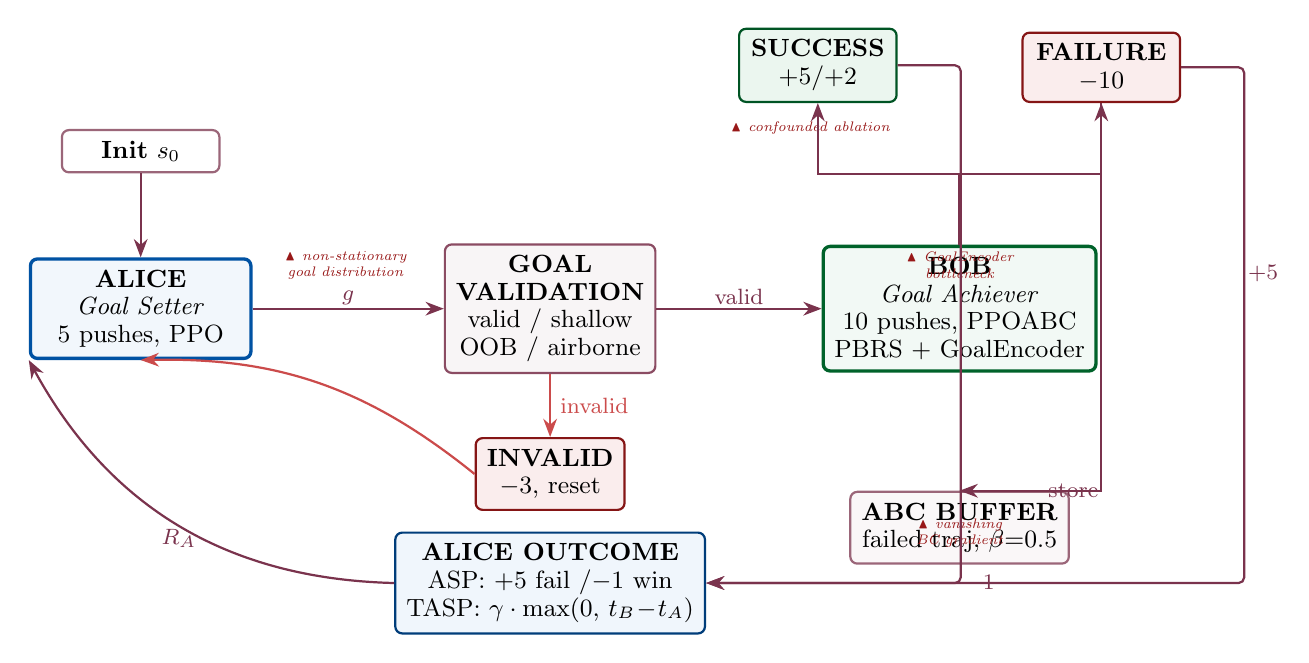
\begin{tikzpicture}[
    box/.style={draw, rounded corners=2.5pt, align=center, inner sep=4pt,
                font=\small, fill=white},
    alice/.style={box, draw=hlblue!80!black, very thick, fill=hlblue!5,
                  minimum width=2.8cm},
    bob/.style={box, draw=hlgreen!70!black, very thick, fill=hlgreen!5,
                minimum width=2.8cm},
    gate/.style={box, draw=DarkBordeaux!70, thick, fill=DarkBordeaux!4,
                 minimum width=2.6cm},
    good/.style={box, draw=hlgreen!60!black, fill=hlgreen!8, thick,
                 minimum width=2.0cm, font=\small},
    bad/.style={box, draw=hlred!70!black, fill=hlred!8, thick,
                minimum width=2.0cm, font=\small},
    rew/.style={box, draw=hlblue!60!black, fill=hlblue!6, thick,
                minimum width=3.6cm, font=\small},
    buf/.style={box, draw=DarkBordeaux!60, thick, fill=DarkBordeaux!3,
                minimum width=2.4cm, font=\small},
    arr/.style={->, >=Stealth, thick, DarkBordeaux!80},
    arrr/.style={->, >=Stealth, thick, hlred!80},
    lbl/.style={font=\footnotesize, DarkBordeaux!80, inner sep=1pt},
]

% --- NODES ---
\node[box, draw=DarkBordeaux!60, thick, minimum width=2.0cm, font=\small]
      (init) at (0, 2.0) {\textbf{Init} $s_0$};

\node[alice] (A) at (0, 0)
    {\textbf{ALICE}\\[-1pt]\textit{Goal Setter}\\[-1pt]
     5 pushes, PPO};

\node[gate] (G) at (5.2, 0)
    {\textbf{GOAL}\\[-1pt]\textbf{VALIDATION}\\[-1pt]
     valid / shallow\\[-1pt]
     OOB / airborne};

\node[bob] (B) at (10.4, 0)
    {\textbf{BOB}\\[-1pt]\textit{Goal Achiever}\\[-1pt]
     10 pushes, PPOABC\\[-1pt]
     PBRS + GoalEncoder};

% Bob outcomes
\node[good, above=1.8cm of B, xshift=-1.8cm] (S)
    {\textbf{SUCCESS}\\[-1pt]$+5$/$+2$};

\node[bad, above=1.8cm of B, xshift=1.8cm] (F)
    {\textbf{FAILURE}\\[-1pt]$-10$};

% Feedback nodes
\node[rew, below=2.0cm of G] (R)
    {\textbf{ALICE OUTCOME}\\[-1pt]
     ASP: $+5$ fail~/$-1$ win\\[-1pt]
     TASP: $\gamma\cdot\max(0,\,t_B\!-\!t_A)$};

\node[buf, below=1.5cm of B] (ABC)
    {\textbf{ABC BUFFER}\\[-1pt]
     failed traj, $\beta{=}0.5$};

\node[bad, below=0.8cm of G, minimum width=1.8cm, font=\small] (inv)
    {\textbf{INVALID}\\[-1pt]$-3$, reset};

% --- FAILURE MODE CALLOUTS ---
\node[font=\tiny\itshape, text=hlred!80!black, align=center, inner sep=2pt]
    at (2.6, 0.55) (f1) {$\blacktriangle$ non-stationary\\goal distribution};

\node[font=\tiny\itshape, text=hlred!80!black, align=center, inner sep=2pt]
    at (10.4, 0.55) (f2) {$\blacktriangle$ GoalEncoder\\bottleneck};

\node[font=\tiny\itshape, text=hlred!80!black, align=center, inner sep=2pt]
    at (10.4, -2.85) (f3) {$\blacktriangle$ vanishing\\BC gradient};

\node[font=\tiny\itshape, text=hlred!80!black, align=center, inner sep=2pt]
    at (8.5, 2.3) (f4) {$\blacktriangle$ confounded ablation};

% --- ARROWS ---
\draw[arr] (init) -- (A);

\draw[arr] (A) -- (G)
    node[lbl, midway, above] {$g$};

\draw[arr] (G) -- (B)
    node[lbl, midway, above] {valid};

\draw[arr, hlred!80, thick] (G) -- (inv)
    node[font=\footnotesize, hlred!80, midway, right] {invalid};

\draw[arr] (B.north) -- ++(0,0.9) -| (S.south);
\draw[arr] (B.north) -- ++(0,0.9) -| (F.south);

\draw[arr, rounded corners=2pt] (S.east) -- ++(0.8,0) |- (R.east)
    node[lbl, pos=0.5, right] {$-1$};

\draw[arr, rounded corners=2pt] (F.east) -- ++(0.8,0) |- (R.east)
    node[lbl, pos=0.2, right] {$+5$};

\draw[arr] (F.south) |- (ABC.north)
    node[lbl, pos=0.7, right] {store};

\draw[arr, bend left=30] (R.west)
    to node[lbl, midway, below] {$R_A$} (A.south west);

\draw[arr, hlred!80, thick, bend right=20] (inv.west) to (A.south);

\end{tikzpicture}
\end{document}
